\section{セキュリティ}
これまで,TCP/IP によるネットワークの構築を行い,多くのネットワークサービスを立ち上げ,
利用者の利便性の向上につながるネットワークシステムの構築を行ってきた.

ルーティングを行い TCP/IP の接続性を向上させ,DNS, Web, 電子メールシステ
ムを構築することで,インターネットを通して世界中から接続可能なネットワー
クサービスの構築を行った.同時に,ファイル転送・ファイル共有などの仕組み
を構築し,情報のやりとりの利便性も向上した.

これまでのネットワークサービスの構築においても,端末ごとのOSのアップデー
トやウイルス対策,サービスごとのアクセス制限など,個々のコンピュータやサー
ビス単位でのセキュリティの設定を行ってきた.

大規模ネットワークの管理を行う場合でも,全ての端末に対して常に万全のセキュ
リティを求めることは重要であるが,セキュリティホール1つからネットワーク
の端末全体の危険が誘発されるような事態も起こり得ることや,多重保護の観点
からもネットワーク単位でのセキュリティも重要となる.

このような目的でネットワーク全体の保護に用いられるセキュリティ技術として,
ファイアウォール(防火壁)がある.ファイアウォールは,ネットワークの入口
で,セキュリティ上好ましくない通信や,不必要な通信を遮断し,アクセス制限
を行う.ファイアウォールには,ネットワーク外部からの攻撃などを遮断する意
図の他,ネットワーク内部からの外部へ向けての攻撃などを防ぐ意図など
もある.具体的には,外部からの攻撃を誘発したり助けたりするような内部から
外部へ向けてのアクセスや,ウイルスなどに感染した内部ホストからの外部への
攻撃をネットワークの入口で防ぐ意図がある.

\section{ファイアウォール}
%本課題では,ファイアウォールの構築を行う.
ファイアウォールは,ネットワークのアクセスを選別し必要のあるアクセスの
みを通過させ,そうでないアクセスを遮断する技術である.

ファイアウォールを用いることによりネットワーク・セキュリティを向上させ
ることができる.しかし,ファイアウォールを構築するだけですべての攻撃を
防ぐことはできない.例えば,ファイアウォールではメールに添付されている
コンピュータウィルスを除去することはできない.また,Web サーバに対して
行なわれる正常な http アクセスを装った DDoS 攻撃\footnote{distibuted
  denial of service の略.複数の拠点から標的のサーバへ一斉に DoS 攻撃を
  仕掛ける.}には対処できない.そして,新しい脅威に対しては,防御できな
い場合も十分に考えられる.そのため,ファイアウォールの運用においては必
ず他のセキュリティ技術と組み合わせることが必要である.

\subsection{ファイアウォールの種類}
ファイアウォールには,大きく分けて次の二種類がある.これは,パケット処
理を行うネットワークレイヤーによる違いである.

\subsubsection{パケットフィルタリングファイアウォール}
図\ref{fig:26:pf}に示すように,内部ネットワークと外部ネットワークの境界
に位置するルータにおいて,パケットフィルタリングルールに従って,二つのネッ
トワーク間でのパケット転送を制御する.宛先IPアドレス・送信元IPアドレス,
プロトコルの種類やポート番号等,IP・TCP・UDP ヘッダの情報に基づく制御
を行う.パケット毎に処理を行い,データの塊や接続状態などは基本的に感知し
ない\footnote{ファイアウォール専用製品(Checkpoint や Cisco,
Juniper(Netscreen) などが有名) ではステートフルインスペクションと呼ばれ
る状態を加味したパケットフィルタも行えるが,処理が複雑になり性能を出すた
めにはより計算性能が求められる.}.


\subsubsection{アプリケーションゲートウェイファイアウォール}
図\ref{fig:26:ag}に示すように,アプリケーション層において,定められたルー
ルに従ってパケットを中継する,あるいは拒否するファイアウォールである.こ
のため,アプリケーションごとの制御や,データ単位での制御,ユーザ単位での
制御が行え,パケットフィルタリングよりもきめ細かい制御が可能となる.実際
の接続を,このゲートウェイが代行することになるので,プロキシ(Proxy:代理)
とも言う.

DNSのキャッシュサービス,電子メールの SMTP サービスも,クライアントの要
求をサーバが代行して行うという点で,一種のアプリケーションゲートウェイで
ある.

ウェブプロキシは,データをいったんサーバにダウンロードし記憶装置に記録す
ることになるため,ウェブキャッシュの機能も持つ.キャッシュの機能を活用す
ることで,多くのユーザがダウンロードを要求するデータは,一度ダウンロード
しキャッシュしたものをユーザに提供することで,インターネット回線の使用帯
域を低減する効果もある.ただし,リアルタイムストリーミングや SSL で暗号
化された接続は,プロキシ機能のみでキャッシュすることはできない.

近年では,パケットフィルタとアプリケーションゲートウェイを組み合わせるパ
ターンが多くなっている\footnote{実際には,内側(trust側),外側(untrust側)
をパケットフィルタで分離し,さらに,内側と外側の両方からアクセス可能な
DMZ (非武装地帯) を作成して,プロキシやメールサーバなどのアプリケーショ
ンゲートウェイとなるサーバをここに設置する.}.ここでは,パケットフィル
タで内側 (trust側) と外側 (untrust側) の通信を完全に遮断し,サーバだけは
外部との必要な通信を許可し,内側の PC からは,サーバのプロキシやメールサー
ビス・DNS サービスを経由して外側のサービスを受信できるようにする.

このように,LAN の一部を完全に外部から遮断する形を,スクリーニングと呼ぶ
場合もある.

\begin{figure}[h]
 \begin{center}
  \resizebox{!}{4cm}{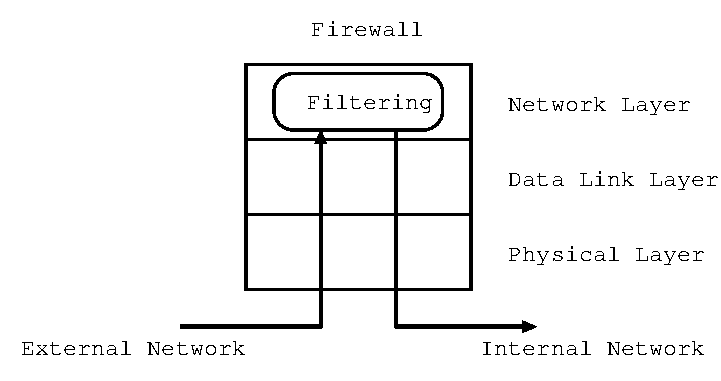
\includegraphics{./security/fw1.eps}}
  \caption{パケットフィルタリング}
  \label{fig:26:pf}
 \end{center}
\end{figure}

\begin{figure}[h]
  \begin{center}
   \resizebox{!}{4cm}{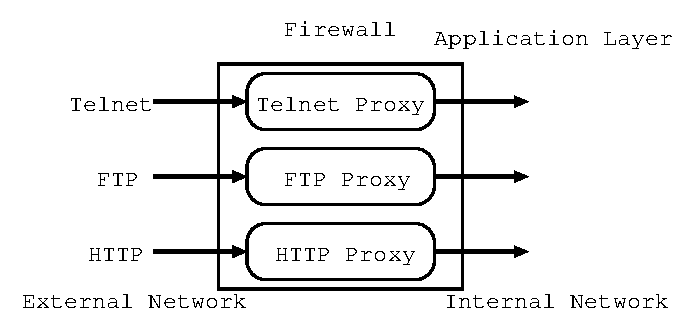
\includegraphics{./security/fw2.eps}}
  \caption{アプリケーションゲートウェイ}
  \label{fig:26:ag}
 \end{center}
\end{figure}

\section{実験内容}
本章において必要となる作業は下記に示すが,まずそれに先だって,NAT の設定
を消去し,NAT を行う前の状態に戻す.
\begin{itemize}
  \item ルータ上でのパケットフィルタ設定
  \item HTTP Proxyサーバの構築
\end{itemize}
である.
本実験では,LANの入口のルータにてパケットフィルタを行う.
パケットフィルタは,サーバ以外の端末は外部との通信を一切不可にし,サーバは外部との通信に必要なもののみを許可する.
内部のPCのネットワークサービスは,全てサーバを通して行う.
メールサービス,DNSサービス,NTPサービスは既にサーバを経由して行っているため,サーバが外部と通信できればサービスに支障はない.
ウェブブラウジングに関しては,現状は各クライアントコンピュータが外部と通信を行うため,パケットフィルタによって通信が遮断されてしまう.
そこで,サーバにてウェブサービスのアプリケーションゲートウェイである,ウェブプロキシを導入する.
本実験でのネットワーク構成を図\ref{fig:26:packet-filter}に示す.

\begin{figure}
  \centering
  \resizebox{!}{8cm}{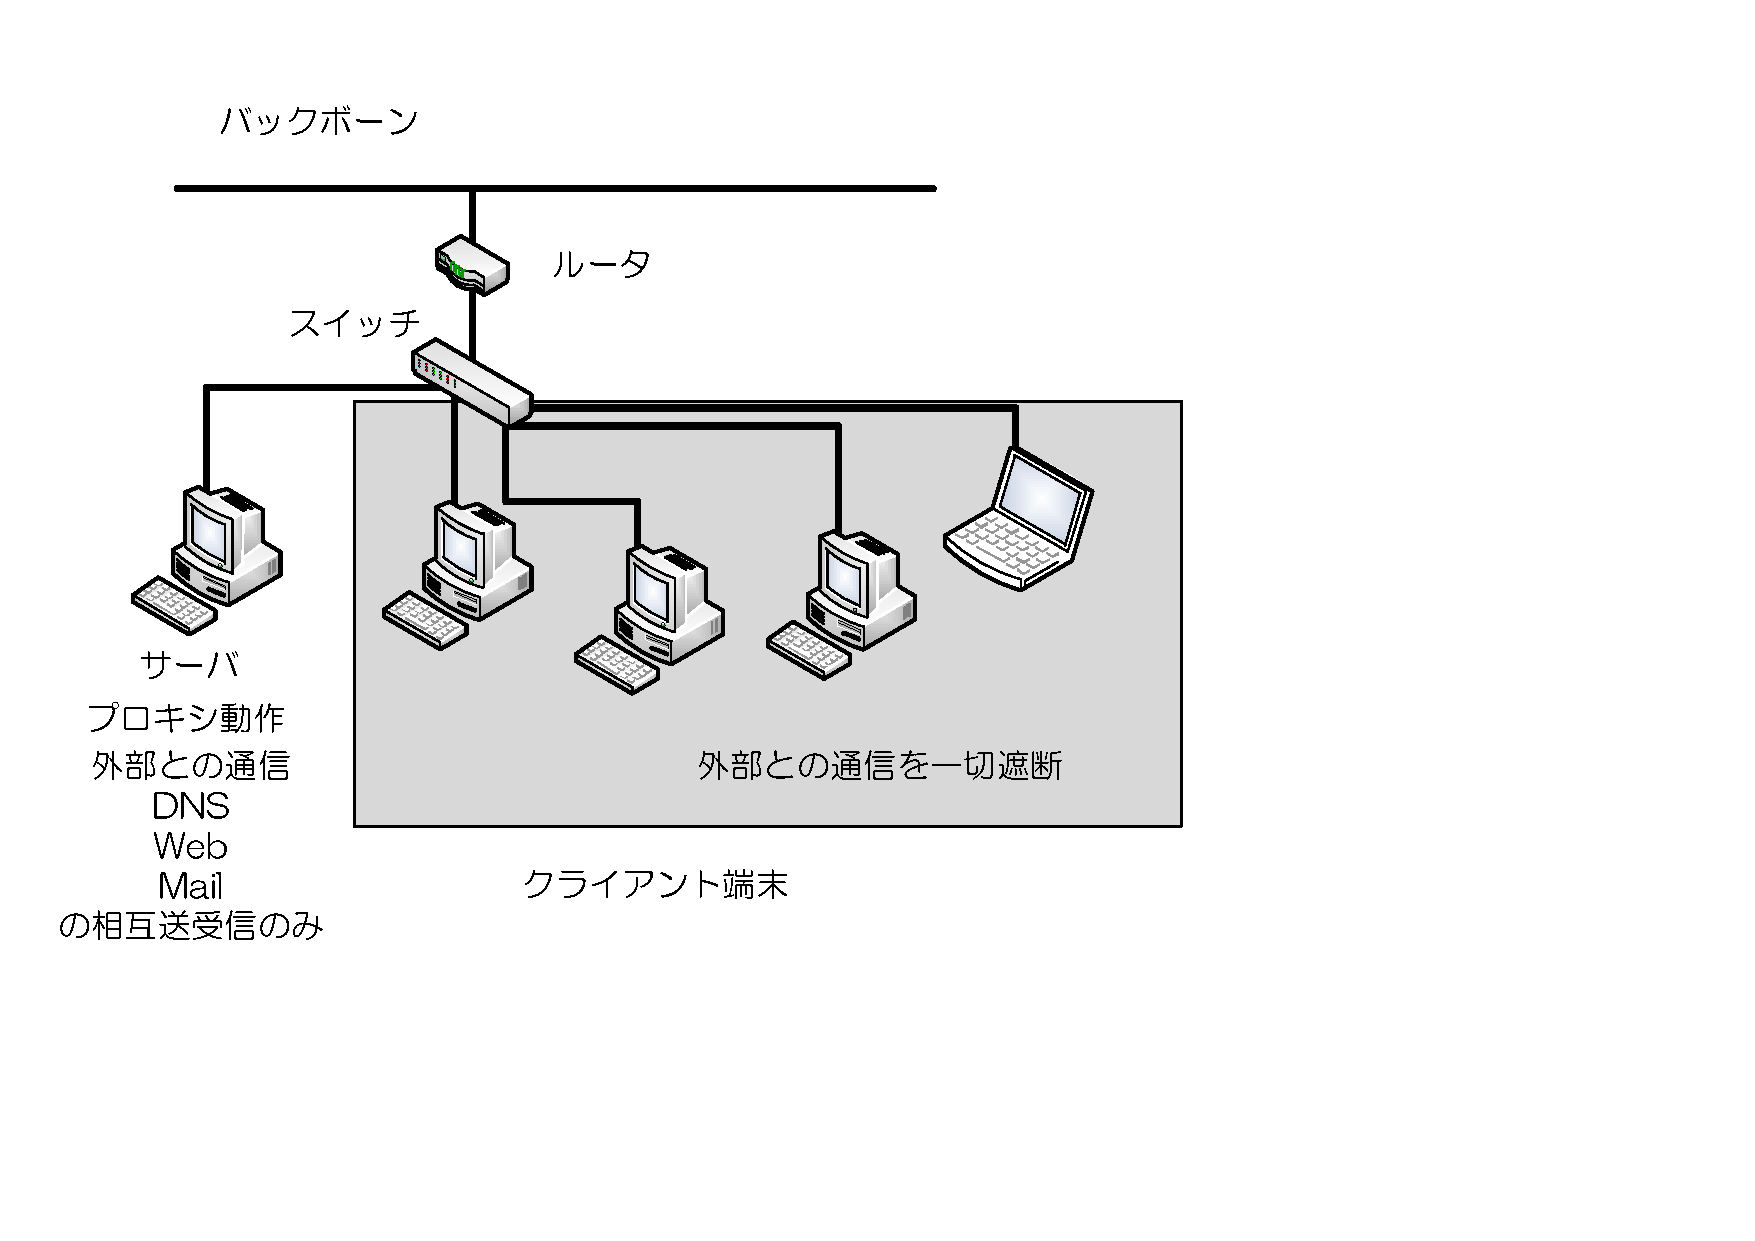
\includegraphics[width=15cm,bb=0 0 720 560,clip]{./security/packetfilter.pdf}}
  \caption{ネットワークの構成図}
  \label{fig:26:packet-filter}
\end{figure}

\section{必要となる知識}
\subsection{パケットフィルタリング}
%まず,入口のルータにてパケットフィルタを構築する.

\subsubsection{Cisco IOS アクセスコントロールリスト}
Cisco 社製ルータに搭載されている IOS には,アクセスコントロールリスト
(Access Control List = ACL,単にアクセスリストとも呼ぶ) と呼ばれるアクセ
ス制限を行う機能があり,この ACL を用いてパケットフィルタリングを行う.

\subsubsection{アクセスリスト}
アクセスリストには,標準アクセスリストと拡張アクセスリストの2種類が存在
する.標準アクセスリストでは,送信元 IP アドレスのみを見てパケット通過の
可否を判断する.これに対して,拡張アクセスリストでは下記に示すようにヘッ
ダの様々な情報を用いて可否を判断する\footnote{なお,宛先IPアドレスのみで
パケットフィルタを行う場合は,ルーティングを用いれば良い.パケット破棄を
行いたい宛先ネットワークに対して,Next hop インターフェースとして, 
Null0 インターフェースを指定した経路を作成することで,パケットが破棄され
る}.
\begin{itemize}
 \item 送信元 IP アドレス
 \item 宛先 IP アドレス
 \item TCP,UDP,ICMP,GRE,その他の IP プロトコルの種類
 \item TCP や UDP の送信元・宛先ポート番号
 \item 送信元・宛先 MAC アドレス
 \item ICMP タイプ・コード
 \item TCP のオプション
\end{itemize}

標準アクセスリストでは,単純に送信元 IP アドレスのみを見れば良いような単
純なルールに用いられる.具体的には,攻撃ホストとして認定されているような
インターネット上の IP アドレスからのアクセスを拒否する場合や,ウイルス感
染が確認された内部ホストからのパケットを拒否する場合などに用いる.拡張ア
クセスリストは,サービス毎に細かい処理をする必要がある場合に使用する.

アクセスリスト番号が1-99までのものは標準アクセスリスト,100-199までは拡
張アクセスリストとして認識される.ルータは通常,外向きのインターフェース
と内向きのインターフェースがあり,外部から内部へのパケットの遮断を行う場
合は外向き側のインターフェースにアクセスリストを,内部から外部へのパケッ
トの遮断を行う場合は内向き側のインターフェースにアクセスリストを用いる.
どちらのアクセスリストの場合でも,アクセスリストを作成した場合に最後に全
て拒否するという暗黙の設定が入るので,基本的には必要なものを許可していく
という方針でアクセスリストを作成する.

\subsubsection{拡張アクセスリストの書式と設定方法}

\begin{cli}
[拡張ACL書式]
access-list  リスト番号  アクション  プロトコル
(続き) 送信元IPアドレス  送信元ワイルドカードマスク [eq  送信元ポート番号]
(続き)   宛先IPアドレス    宛先ワイルドカードマスク [eq    宛先ポート番号]
(続き)   [established] [icmp type] [icmp code]
\end{cli}

\begin{itemize}
 \item ブラケット[]内は省略することができる.
 \item リスト番号は,ひとまとまりのアクセスリストに対して同じ番号(100~199)を
付与する(1~99: 標準ACL⇒送信元IPのみで判断,100~199: 拡張ACL⇒IP・TCP・
       UDPヘッダ)
 \item アクション→permit (許可) or deny(拒否)
 \item プロトコル→ip(すべてのIPパケット),tcp,udp,icmp
 \item ポート番号→UDP・TCPの時のみ有効.ポート番号を指定.省略した場合ポート番号の検査は行わない
(すべてのポート番号が該当する).
 \item established→TCPの時のみ有効.ACKフラグのあるパケットを照合.
 \item icmp type→ICMPの時のみ有効.ICMPタイプ番号を指定.
 \item icmp code→ICMPの時のみ有効.ICMPコード番号を指定.
\end{itemize}

このようなパケット照合のパターンを複数行続けて書いたものがアクセスリスト
である.パケットの照合はリストの上から順に行われ,最初にマッチしたパター
ンのアクションが実行され,この後のリストは評価されない.最後まで照合を行っ
てもマッチしなかったパケットは破棄される.これを,最後の行に deny の行が
あるような振舞いであることから,暗黙のdeny と呼ぶ.

送信元 IP アドレス・宛先 IP アドレスは,ワイルドカードを設定することによ
り,複数のアドレスをまとめて指定することが可能である.ワイルドカードマス
クは,IPアドレスを32ビットの2進数表記にした際,チェックを行うビットは0,
チェックを行わないビットは1とし,8ビット毎にドットで区切った10進数4つで
表す.

例えば,172.21.39.0 〜 172.21.39.255を指定する場合は,172.21.39.0
0.0.0.255 とする.0.0.0.0 255.255.255.255とした場合は,任意の IP アドレ
スを意味し,これは any と書いても良い.また,単一のIPアドレスのみを照合
する場合,"IPアドレス  0.0.0.0" とする.これは,"host  IPアドレス" と書いて
も良い.

次に,定義したリストを ip access-group コマンドでインターフェースに設定する.

\begin{cli}
interface fastethernet0
  ip access-group リスト番号 in(out)
\end{cli}

この例は,リスト番号のアクセスリストを,fastethernet0 からパケットが入っ
て来る(in)際(あるいは,出て行く際 (out)) 評価する設定である.

\subsubsection{アクセスリストの設定}
アクセスリストの設定は Windows PC とルータをシリアルケーブルで接続し,ター
ミナルソフトウェア Putty を用いて行う.ターミナルの設定方法などは以前行っ
ているので割愛する.

まず,テキストエディタで次のようなファイルを作成しておく.

\begin{center}
\begin{breakbox}
\begin{alltt}
[[100番のリストは,外側インターフェース向け]]
no access-list 100

  ↓ インターネットからサーバへの DNS 問い合わせを許可
access-list 100 permit udp any host 172.21.X.2 eq 53
access-list 100 permit tcp any host 172.21.X.2 eq 53

  ↓ インターネットからサーバへの SMTP 接続を許可
access-list 100 permit tcp any host 172.21.X.2 eq 25

  ↓ インターネットからサーバへの HTTP(SSL) 接続を許可
access-list 100 permit tcp any host 172.21.X.2 eq 80
access-list 100 permit tcp any host 172.21.X.2 eq 443

  ↓ インターネットからルータへの着信を許可
     さらにブロードキャストも許可,
access-list 100 permit ip any host 192.168.0.X
access-list 100 permit ip any host 192.168.0.255
access-list 100 permit ip any host 255.255.255.255

  ↓ インターネットからルータへの OSPF
     マルチキャスト着信を許可
access-list 100 permit ip any host 224.0.0.5
access-list 100 permit ip any host 224.0.0.6

  ↓ インターネットからサーバへの DNS 問い合わせ,
     SMTP 接続,HTTP(S)接続に対する応答パケットの許可
access-list 100 permit udp any eq 53 host 172.21.X.2
access-list 100 permit tcp any eq 53 host 172.21.X.2
access-list 100 permit tcp any eq 25 host 172.21.X.2
access-list 100 permit tcp any eq 80 host 172.21.X.2
access-list 100 permit tcp any eq 443 host 172.21.X.2


[[101 番のリストは,内側インターフェース向け]]
(それぞれの意味をよく考える.
no access-list 101
access-list 101 permit udp host 172.21.X.2 any eq 53
access-list 101 permit tcp host 172.21.X.2 any eq 53
access-list 101 permit tcp host 172.21.X.2 any eq 25
access-list 101 permit tcp host 172.21.X.2 any eq 80
access-list 101 permit tcp host 172.21.X.2 any eq 443
access-list 101 permit udp host 172.21.X.2 eq 53 any
access-list 101 permit tcp host 172.21.X.2 eq 53 any
access-list 101 permit tcp host 172.21.X.2 eq 25 any
access-list 101 permit tcp host 172.21.X.2 eq 80 any
access-list 101 permit tcp host 172.21.X.2 eq 443 any
\end{alltt}
\end{breakbox}
\end{center}

このリストをルータを接続したターミナルソフトウェアにて,configure
terminal を行った状態ではりつける.

次に,ルータでインターフェースへの適用を行う.
\begin{center}
\begin{breakbox}
\begin{alltt}
CiscoX% en
CiscoX# conf term
CiscoX(config)# interface FastEthernet0
CiscoX(config-if)# ip access-group 100 in
                (外向けのインタフェースFastEthernet0に外部から入ってくるパケットに対しアクセスリスト100を適用する)
CiscoX(config-if)# end
CiscoX(config)# interface FastEthernet1
CiscoX(config-if)# ip access-group 101 in
                (内向けのインタフェースFastEthernet1に内部から入ってくるパケットに対しアクセスリスト101を適用する)
CiscoX(config-if)# end
\end{alltt}
\end{breakbox}
\end{center}

アクセスリストは上から順にルールがチェックされ,最初に適合したルールが実
行されて終了する.

(ソフトウェアの if-else if-else if ... 構造と同様).

そのため,順序も意味を持ってくる.

アクセスリストの消去は,下記のコマンドで行う.
\begin{center}
\begin{breakbox}
\begin{alltt}
CiscoX(config)# no access-list XXX(消したいアクセスリスト番号)
\end{alltt}
\end{breakbox}
\end{center}
同様に,インターフェースに対するアクセスグループを消したい場合には以下のようにする.
\begin{center}
\begin{breakbox}
\begin{alltt}
CiscoX(config)# no ip access-group XXX in
\end{alltt}
\end{breakbox}
\end{center}



%                      ファイアーウォールの構築
%                                        written by T.Nakahira
%                                        modified by Y.Komatsu
%
%                                          Last updated: 2004/03/24
\subsection{HTTP Proxy}
アクセスリストの設定により,サーバ以外の端末は LAN の外へ直接通信ができ
なくなっている.電子メールは,SMTPサーバ,POPサーバとも サーバ を経由し,
DNS もサーバを経由するようになっており,サーバ 以外の端末は LAN 外への通
信は行わない.しかし,Web 閲覧は各端末とも直接外部へ HTTP 通信を行う.
HTTP 通信もサーバ で経由して行わせるために,サーバ 上へプロキシサービス
をインストールする.

HTTP プロトコルに対して Proxy 機能を実装したフリーのソフトウェアとし
て,Squid,Delegate, Apache などがあるが,一般的に広く使われているものは Squid である.
%ため,本実験では Squid のインストールを行う.
Squid は,Harvest プロジェクトで基本的な開発が行われ,現在では
NLANR\footnote{National Laboratory for Applid Network Research} を中心
に開発が行われている.

本節では,Squid を用いて HTTP Proxy を構築する方法を述べる.

\subsubsection{Squid のインストール・設定}

インストールはこれまでのオープンソースソフトウェアの構築手順とほぼ同様で
あり,アーカイブ中の INSTALL ファイルを読んで進めれば良い.

squidの設定は,/usr/local/squid/etc/squid.conf ファイルを編集することで行う.
設定する前に,オリジナルをコピーしておく.

\begin{center}
\begin{breakbox}
\begin{alltt}
server# cd /usr/local/squid/etc
server# cp -p squid.conf squid.conf.org
server# vi squid.conf
\end{alltt}
\end{breakbox}
\end{center}

\subsubsection{キャッシュ(Cache)の設定}
%続いてキャッシュ (Cache) の設定を行う.
%
キャッシュとは,データを一時的に蓄積することである.
クライアントが要求したデータが蓄積データに存在した場合,本来の宛先コンピュータに代わって
そのデータをクライアントに返送することで,ネットワークトラフィックを減少させ,回線容量が圧迫されるのを
防ぐことができる.同時に,クライアントは短時間で目的データを得ることができる.

Squid は Proxy の機能と同時に キャッシュサーバとしても動作することが可能である.
ここでは,プロキシをセキュリティの向上を目的に導入しているが,本来,プロ
キシは,セキュリティの向上とともに,キャッシュによるトラフィックの軽減
も重要な役割である.

\begin{center}
\begin{breakbox}
\begin{alltt}
server# cd /usr/local/squid/var
server# mkdir cache
server# chown -R nobody:wheel cache
server# chown nobody:wheel ./logs
server# /usr/local/squid/sbin/squid -z   (キャッシュディレクトリが作成される)
\end{alltt}
\end{breakbox}
\end{center}

\subsubsection{Squidの起動}
Squid の起動方法は次の通りである.起動処理が完了するのに,しばらく時間がかかる.

\begin{center}
\begin{breakbox}
\begin{alltt}
server# /usr/local/squid/sbin/squid
\end{alltt}
\end{breakbox}
\end{center}

%Squid の起動確認は,次のように ps コマンドで行う.
%
%\begin{center}
%\begin{breakbox}
%\begin{alltt}
%server# ps ax | grep squid
%\end{alltt}
%\end{breakbox}
%\end{center}

\section{必要な情報}
\subsection{Squid.confの設定}
squid.conf の設定例を以下に示す.
ファイル内にそれぞれ該当する行がある場合は,行頭の \# (コメントアウト)を取り除いて有効にし,適切な値を書き込む.
無い場合は新たに書き加える.

% \begin{description}
%  \item[http\_port] Proxy のポート番号.Squid デフォルトの 3128 で良い.
%  \item[acl] アクセスコントロールリスト.
% \begin{cli}
% acl  名前  src|dst  X.Y.Z.W/PRE
%   名前という形で,プレフィックス表記の IP アドレスブロック X.Y.Z.W/PRE
%   を送信元(src)または宛先(dst) とするパケットを定義する.
% acl  Safe\_ports  port  X
%    ポート番号 X での(Proxyによる代理)通信を行う.
% http\_access  allow|deny  名前
%    名前で定義したアドレスに関する通信を許可(allow)または拒否(deny)する.
% cache\_dir ufs dir 100 16 256
%     キャッシュディレクトリを dir に設定する.
%     16, 256 などは,同一ディレクトリ内のサブディレクトリやファイルの数を
%     決める.ファイルシステムによっては,同一ディレクトリ内のファイル数が
%     増えすぎるとアクセス速度が極端に低下するため.

%     注意:キャッシュの大きさを調整すること.特に容量の少ないSSDなどでは
%           注意する.
% \end{cli}
% \end{description}

\paragraph{squid.conf の説明}
\begin{itemize}
\item http\_port \textless port\textgreater \ \\
HTTPリクエストを受けるポート番号の指定
\item icp\_port \textless port\textgreater \ \\
ICPリクエストを受けるポート番号の指定
\item acl \textless aclname\textgreater \textless acltype\textgreater \textless hostname\textgreater \textless hostname\textgreater
    \begin{itemize}
    \item \textless aclname\textgreater :任意の文字列をアクセス制御リスト名として指定
    \item \textless acltype\textgreater  :\textless hostname\textgreater のタイプを指定
    \item \textless hostname \textbar  filename\textgreater :ホスト名または IP アドレスを指定
    \end{itemize}
\item http\_access allow \textless aclname\textgreater \ \\
acl タグで指定したアクセス制御対象に対してアクセスを許可
\item cache\_mgr \textless address\textgreater \ \\
squid のエラーメールを受け取るアドレスを指定.デフォルトでは webmaster となっている
\item cache\_effective\_user \textless username\textgreater \ \\
squidプロセスのユーザ権限を設定.デフォルトでは nobody となっている
\item cache\_effective\_user \textless groupname\textgreater \ \\
squid プロセスのグループ権限を設定.デフォルトでは nogroup となっている
\item cache\_dir \textless directory\textgreater \textless size\textgreater \textless level-1\textgreater \textless level-2\textgreater
    \begin{itemize}
    \item \textless directory\textgreater :キャッシュファイルを保存するディレクトリを指定
    \item \textless size\textgreater :キャッシュ容量をMバイト単位で指定
    \item \textless level-1\textgreater  :1段目のディレクトリ数
    \item \textless level-2\textgreater  :2段目のディレクトリ数
    \end{itemize}
\end{itemize}

\section{作業の概要}
%\subsection{セキュリティポリシー}
ルータによるアクセスリストを用いセキュリティーレベルを向上させる場合,
先にネットワークのセキュリティーに関するポリシーを策定する必要がある.
今回の実験では今後の実験内容も考慮し以下のような構成にする.

\begin{itemize}
 \item サーバ以外のコンピュータ:内部ネットワーク ←→ 外部ネットワーク
       の通信を全て遮断.それぞれ,サーバの DNSキャッシュ・MTA・Web プロ
       キシを介しての外部とのやりとりを行うよう設定する.
 \item サーバ: 外部ネットワークとは,DNS, メール送受信,ウェブ送受信を行えるようにする.
\end{itemize}

\section{動作確認}
他グループの端末からルータ,ハブ,サーバ等に ping を行い,通信の可否が期待通りの動作か確認する.
また,自ネットワークから他のネットワークに対しても,通信の可否を確認する.

Squid の起動確認として,適当なホストから WWW ブラウザを起動し,HTTP プロキシを使用するように設定する.
ブラウザの設定において,プロキシサーバはSquidサーバの IP アドレス,ポー
トは \texttt{3128} を指定する.\texttt{http://192.168.0.1/} へアクセスし,
ウェブが表示されることを確認する.また,プロキシを使用しない場合には,ウェ
ブが表示されないことも確認する.

\section{考慮すべき点}
今回の実験を行うに当たっては以下のようなことについて考慮する必要がある.

\paragraph{ファイアウォールの種類}
パケットフィルタ・アプリケーションゲートウェイには,それぞれ処理速度・細
かな制御という利点があるが,これらの他のタイプのファイアウォールを考える
ことはできるか.

\paragraph{プロキシ}
アクセスを制限するホストはどのように決定すればよいか.またプロキシは,
キャッシュとしての機能も持つが,その他にプロキシを導入することに対する利
点あるいは欠点はあるか.
